\input{preamble.tex}

\title{Отчет по лабораторной работе № 1. \\ Знакомство с Cisco Packet Tracer}
\author{Сущенко Алина \\ НПИбд-01-23}
\date{2026}

\begin{document}

\maketitle
\newpage

\tableofcontents

\newpage
\section{Цель работы}
Установить инструмент моделирования конфигурации сети \texttt{Cisco Packet Tracer}, ознакомиться с его интерфейсом.

\newpage
\section{Выполнение работы}

\subsection{Запуск Cisco Packet Tracer без использования сетевого соединения}
\begin{enumerate}
\item Для ОС типа Windows блокируем для \texttt{Packet Tracer} доступ в Интернет (Рис. \ref{01}-\ref{02}):
Для этого в дополнительных параметрах Брандмауэра создаём своё правило. Для нашего случая:
  \begin{minted}{bash}
  Выбираем «Для программы» и нажимаем «Далее».
  Указываем путь к исполняемому файлу программы, которой нужно запретить доступ в Интернет. В данном случае путь к установленному ОС Packet Tracer, а именно к исполняемому файлу.
  В следующем окне оставим отмеченным пункт «Блокировать подключение».
  В следующем окне отметим, для каких сетей выполнять блокировку.
  Укажем понятное имя правила и нажмём «Готово».
  \end{minted}
  \begin{center}
    \centering
    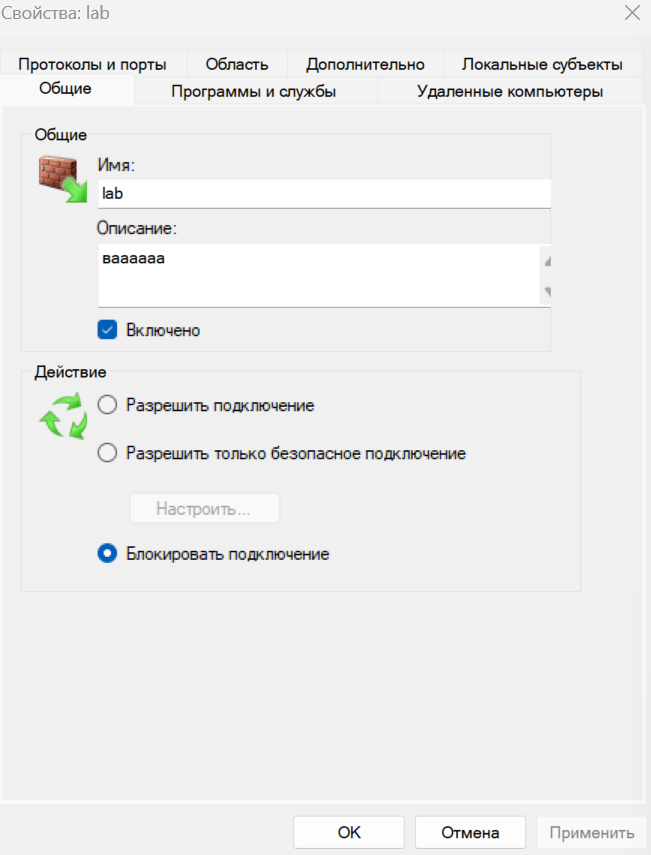
\includegraphics[width=\textwidth]{../images/01.png}
    \captionof{figure}{Конечная настройка подключения к сети (часть с ограничением подключения).}
    \label{01}
\end{center}
  \begin{center}
    \centering
    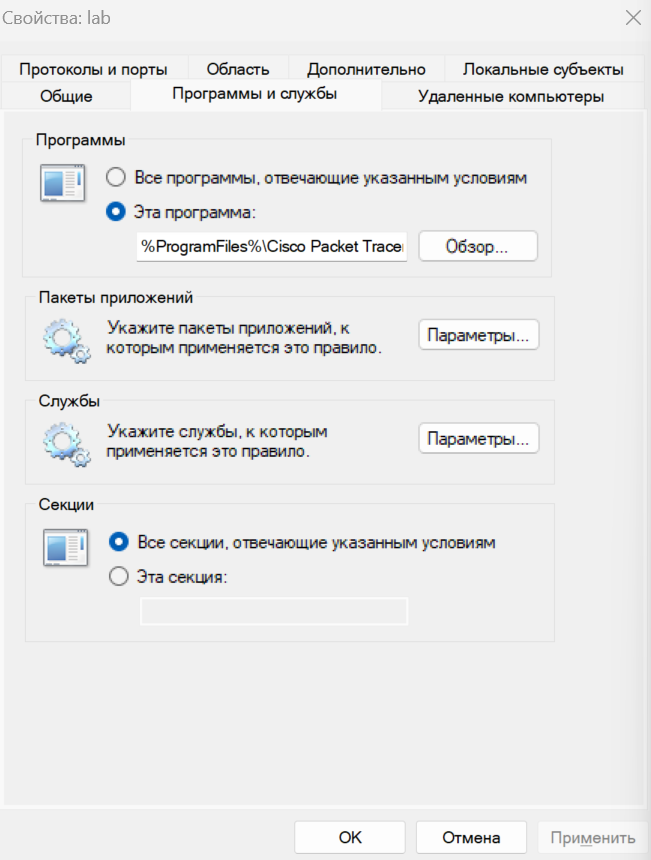
\includegraphics[width=\textwidth]{../images/02.png}
    \captionof{figure}{Конечная настройка подключения к сети (часть с расположением файла на компьютере).}
    \label{02}
\end{center}
\end{enumerate}

\subsection{Знакомство с интерфейсом Packet Tracer}
Первоначальную настройку осуществили, \texttt{Cisco Packet Tracer} открылся без просьбы логина.

\begin{enumerate}
\item Ознакомились с рабочим пространством (Рис. \ref{03}):
\begin{center}
    \centering
    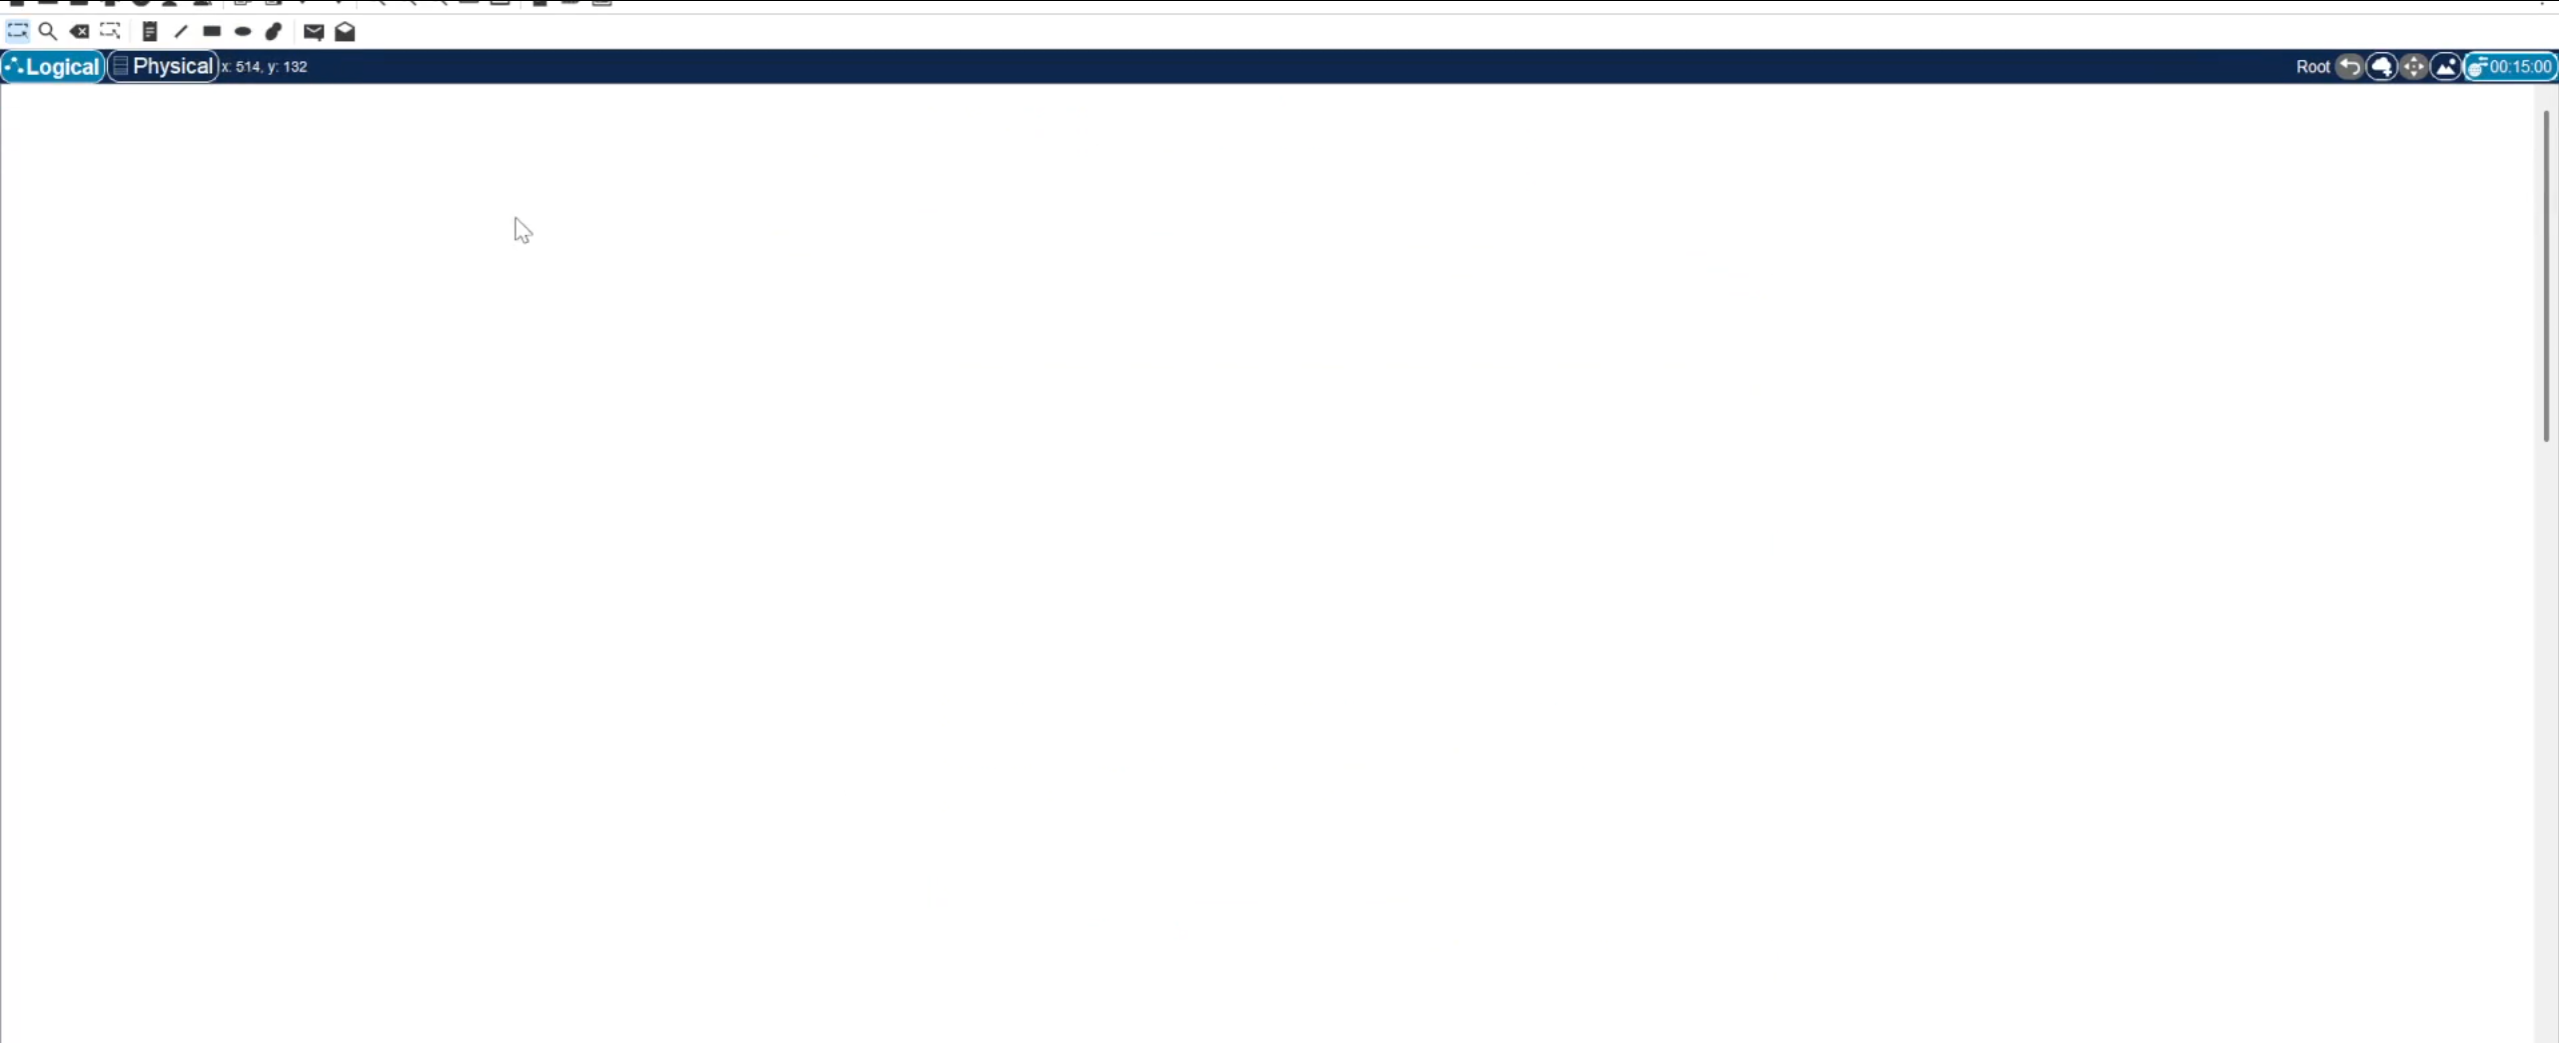
\includegraphics[width=\textwidth]{../images/03.png}
    \captionof{figure}{Чистое рабочее пространство.}
    \label{03}
\end{center}
\end{enumerate}

\subsection{Построение простейшей сети}
\begin{enumerate}
\item Создадим новый проект с названием \texttt{lab\_PT-01.pkt} (Рис. \ref{04}):
\begin{center}
    \centering
    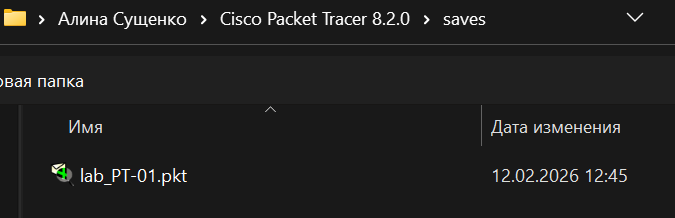
\includegraphics[width=\textwidth]{../images/04.png}
    \captionof{figure}{Созданный проект.}
    \label{04}
\end{center}

\item В рабочем пространстве разместим концентратор Hub-PT и четыре устройства PC. Соединим оконечные устройства с концентратором прямым кабелем (Рис. \ref{05}):
\begin{center}
    \centering
    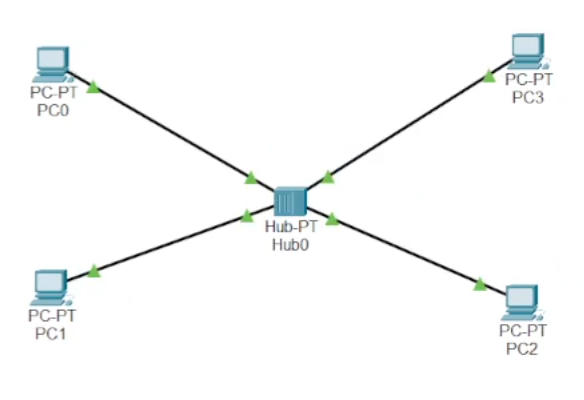
\includegraphics[width=\textwidth]{../images/05.png}
    \captionof{figure}{Модель простой сети с концентратором.}
    \label{05}
\end{center}

\item Щёлкнув последовательно на каждом оконечном устройстве, зададим статические IP-адреса 192.168.1.11, 192.168.1.12, 192.168.1.13, 192.168.1.14 с маской подсети 255.255.255.0 (Рис. \ref{06}, \ref{07}, \ref{08}, \ref{09}):
\begin{center}
    \centering
    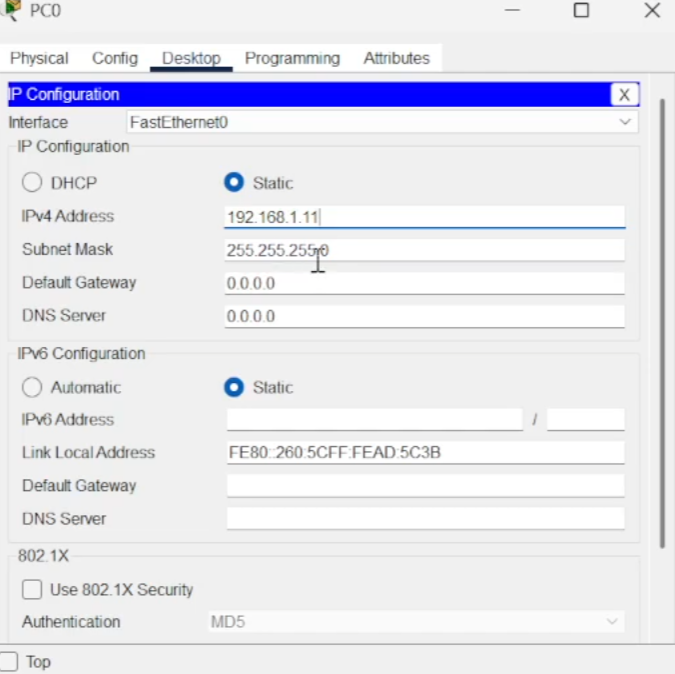
\includegraphics[width=\textwidth]{../images/06.png}
    \captionof{figure}{Статический IP-адрес для PC-PT PC0.}
    \label{06}
\end{center}
\begin{center}
    \centering
    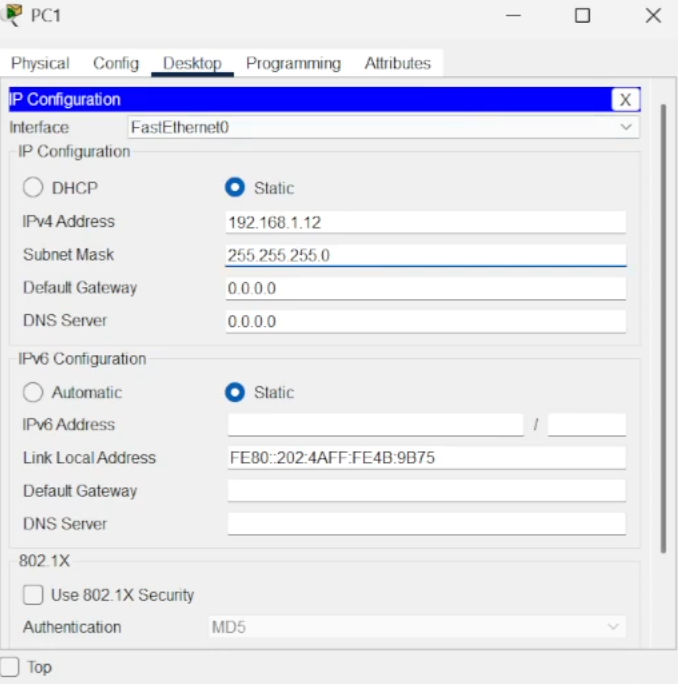
\includegraphics[width=\textwidth]{../images/07.png}
    \captionof{figure}{Статический IP-адрес для PC-PT PC1.}
    \label{07}
\end{center}
\begin{center}
    \centering
    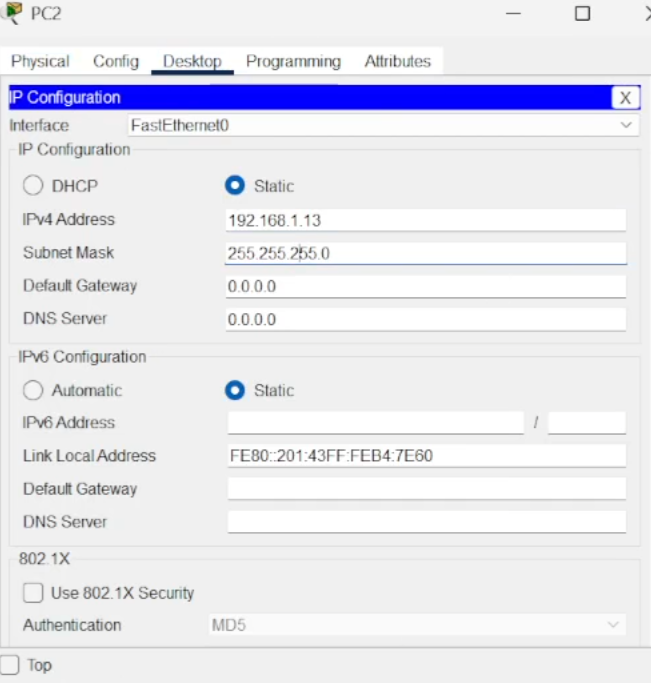
\includegraphics[width=\textwidth]{../images/08.png}
    \captionof{figure}{Статический IP-адрес для PC-PT PC2.}
    \label{08}
\end{center}
\begin{center}
    \centering
    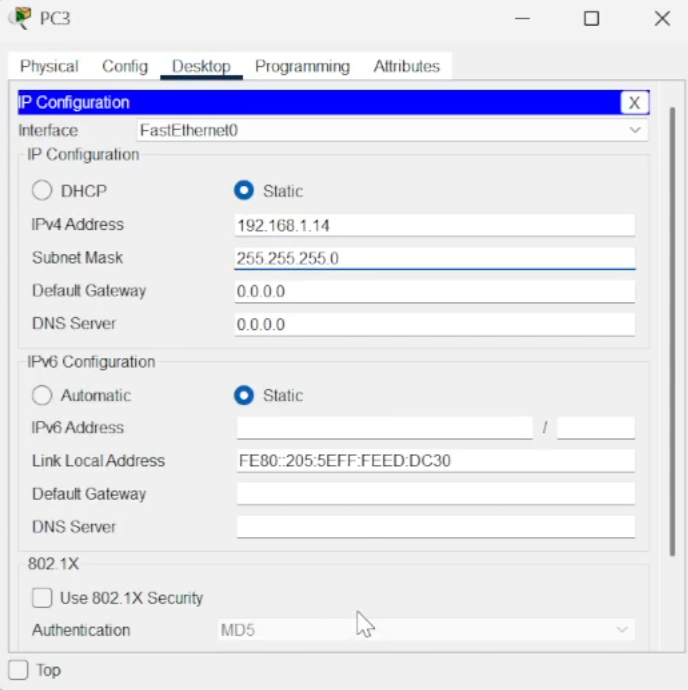
\includegraphics[width=\textwidth]{../images/09.png}
    \captionof{figure}{Статический IP-адрес для PC-PT PC3.}
    \label{09}
\end{center}

\item В основном окне проекта перейдём из режима реального времени (Realtime) в режим моделирования (Simulation). Выберем на панели инструментов «Add Simple PDU (P)» и щёлкнем сначала на PC0, затем на PC2. На панели моделирования нажмём кнопку «Play» и проследим за движением пакетов ARP и ICMP от устройства PC0 до устройства PC2 и обратно (Рис. \ref{10}, \ref{11}):
\begin{center}
    \centering
    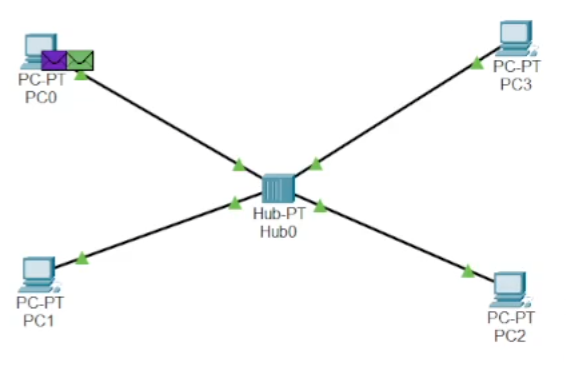
\includegraphics[width=\textwidth]{../images/10.png}
    \captionof{figure}{Два конверта в рабочей области.}
    \label{10}
\end{center}
\begin{center}
    \centering
    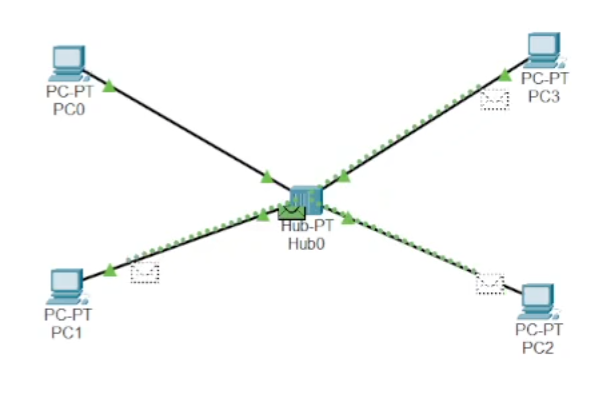
\includegraphics[width=\textwidth]{../images/11.png}
    \captionof{figure}{Движение конвертов.}
    \label{11}
\end{center}

\item Щёлкнем на строку события, откроем окно информации о PDU и изучим, что происходит на уровне модели OSI при перемещении пакета. Там же используем кнопку «Проверь себя» (Challenge Me) на вкладке OSI Model и ответим на вопросы (Рис. \ref{12}, \ref{13}):
\begin{center}
    \centering
    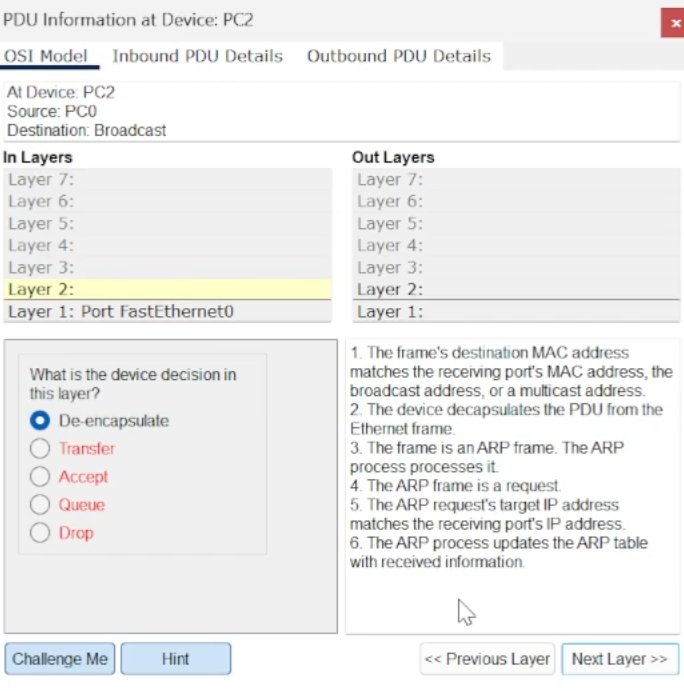
\includegraphics[width=\textwidth]{../images/12.png}
    \captionof{figure}{Вкладка OSI Model и Challenge Me.}
    \label{12}
\end{center}
\begin{center}
    \centering
    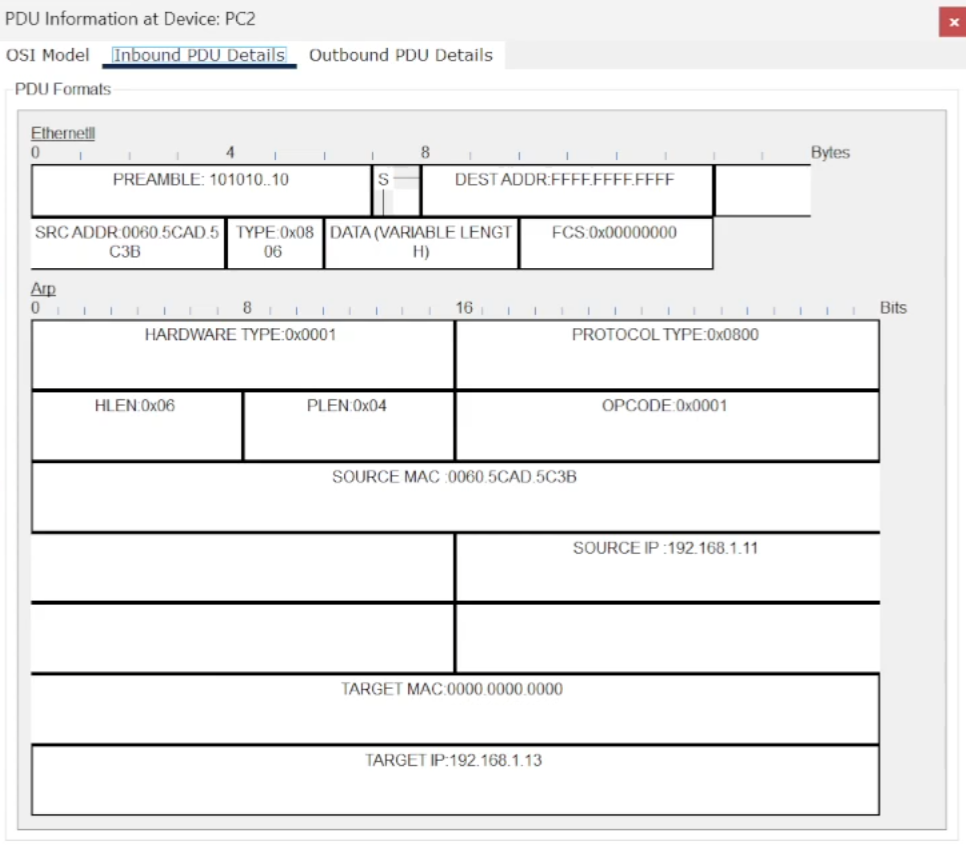
\includegraphics[width=\textwidth]{../images/13.png}
    \captionof{figure}{Вкладка информации о PDU.}
    \label{13}
\end{center}

\item Откроем вкладку с информацией о PDU. Исследуем структуру пакета ICMP.

\subsubsection*{Структура кадра Ethernet}
\begin{center}
\begin{tabular}{|l|l|c|}
\hline
\textbf{Поле} & \textbf{Значение} & \textbf{Длина} \\
\hline
PREAMBLE & 101010…10 & 7 байт \\
SFD & 10101011 & 1 байт \\
DESTADDR & FF:FF:FF:FF:FF:FF & 6 байт \\
SRC ADDR & 0060.5CAD.5C3B & 6 байт \\
TYPE & 0x0806 (ARP) & 2 байта \\
DATA & ARP-запрос (переменная длина) & 28+ байт \\
FCS & 0x00000000 & 4 байта \\
\hline
\end{tabular}
\end{center}

\textbf{Тип кадра:} Ethernet II. Определяется по полю \texttt{TYPE} (0x0806 для ARP, 0x0800 для IPv4, 0x2000 для CDP).

\subsubsection*{Структура MAC-адресов (для ARP-запроса)}
\begin{center}
\begin{tabular}{|l|l|l|}
\hline
\textbf{Адрес} & \textbf{Значение} & \textbf{Описание} \\
\hline
Destination MAC & \texttt{FF:FF:FF:FF:FF:FF} & Широковещательный (broadcast) \\
Source MAC & \texttt{0060.5CAD.5C3B} & MAC-адрес отправителя (PC0) \\
\hline
\end{tabular}
\end{center}

\subsubsection*{Структура пакета ICMP}
ICMP работает поверх протокола IPv4. Кадр Ethernet для ICMP имеет:
\begin{center}
\begin{tabular}{|l|l|c|}
\hline
\textbf{Поле} & \textbf{Значение} & \textbf{Длина} \\
\hline
DESTADDR & MAC-адрес получателя & 6 байт \\
SRC ADDR & MAC-адрес отправителя & 6 байт \\
TYPE & 0x0800 (IPv4) & 2 байта \\
DATA & IP-пакет, внутри ICMP & переменная \\
\hline
\end{tabular}
\end{center}

Структура ICMP-пакета (Echo Request / Echo Reply):
\begin{center}
\begin{tabular}{|l|l|c|}
\hline
\textbf{Поле} & \textbf{Значение} & \textbf{Длина} \\
\hline
Type & 8 (Request) / 0 (Reply) & 1 байт \\
Code & 0 & 1 байт \\
Checksum & Контрольная сумма & 2 байта \\
Identifier & Идентификатор процесса & 2 байта \\
Sequence Number & Номер последовательности & 2 байта \\
Data & Произвольные данные (payload) & переменная \\
\hline
\end{tabular}
\end{center}

\item Теперь очистим список событий, удалив сценарий моделирования. Затем выберем на панели инструментов мышкой «Add Simple PDU (P)» и щёлкнем сначала на PC0, затем на PC2. Снова выберем на панели инструментов мышкой «Add Simple PDU (P)» и щёлкнем сначала на PC2, затем на PC0. На панели моделирования нажмём кнопку «Play» и проследим за возникновением коллизии (Рис. \ref{14}). 

\subsubsection*{Почему возникла коллизия?}
Коллизия возникла потому, что в качестве сетевого устройства используется \textbf{концентратор (Hub-PT)}, который работает на \textbf{физическом уровне (L1)} модели OSI. Концентратор не анализирует содержимое кадров и не буферизирует их, а просто ретранслирует электрические сигналы на \textbf{все порты}, кроме входящего.

При одновременной отправке кадров:
\begin{itemize}
    \item \textbf{PC0} отправляет кадр в сторону \textbf{PC2};
    \item \textbf{PC2} отправляет кадр в сторону \textbf{PC0};
    \item Оба кадра одновременно поступают на \textbf{Hub};
    \item Hub ретранслирует их на все порты;
    \item На среде передачи происходит \textbf{наложение сигналов} — \textbf{коллизия}.
\end{itemize}

\subsubsection*{Как отображается информация о коллизии в заголовках пакетов?}
Коллизия — это \textbf{физическое событие}, которое:
\begin{itemize}
    \item Не записывается в заголовок кадра;
    \item Не передаётся в PDU;
    \item Не видна в полях Destination MAC, Source MAC, EtherType и др.
\end{itemize}

\begin{center}
    \centering
    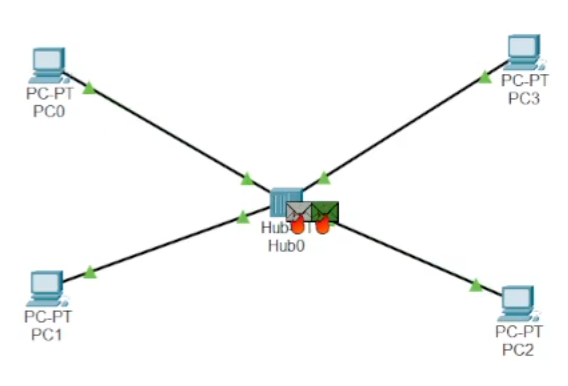
\includegraphics[width=\textwidth]{../images/14.png}
    \captionof{figure}{Коллизия.}
    \label{14}
\end{center}

\item Вернёмся обратно в режим реального времени (Realtime) и добавим новую схему. В рабочем пространстве разместим коммутатор Cisco 2960-24 и 4 оконечных устройства PC. Соединим оконечные устройства с коммутатором прямым кабелем (Рис. \ref{15}):
\begin{center}
    \centering
    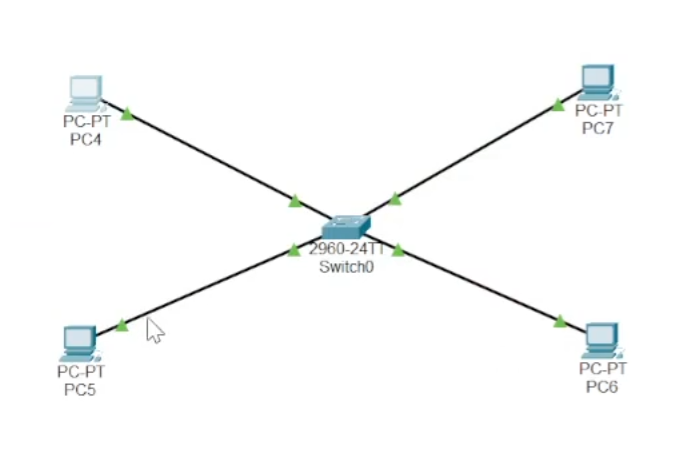
\includegraphics[width=\textwidth]{../images/15.png}
    \captionof{figure}{Модель простой сети с коммутатором.}
    \label{15}
\end{center}

\item Щёлкнем последовательно на каждом оконечном устройстве, зададим статические IP-адреса 192.168.1.21, 192.168.1.22, 192.168.1.23, 192.168.1.24 с маской подсети 255.255.255.0 (Рис. \ref{16}, \ref{17}, \ref{18}, \ref{19}):
\begin{center}
    \centering
    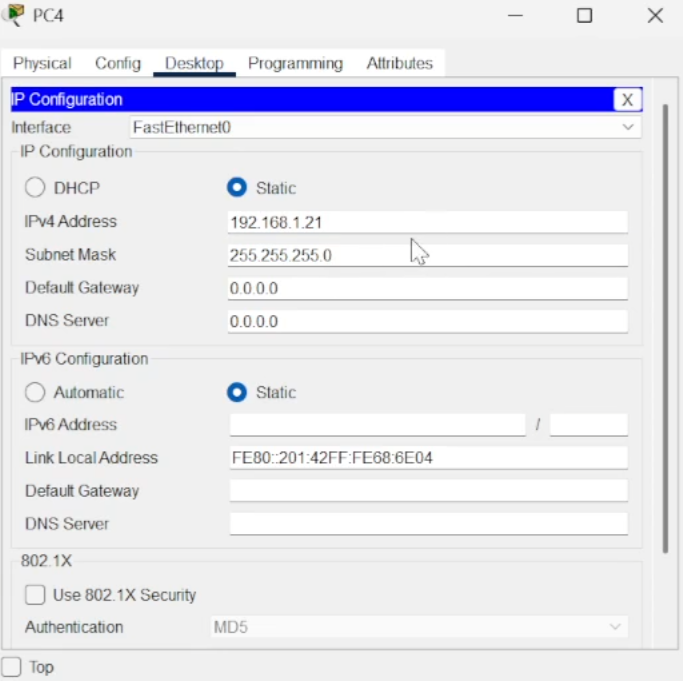
\includegraphics[width=\textwidth]{../images/16.png}
    \captionof{figure}{Статический IP-адрес для PC-PT PC4.}
    \label{16}
\end{center}
\begin{center}
    \centering
    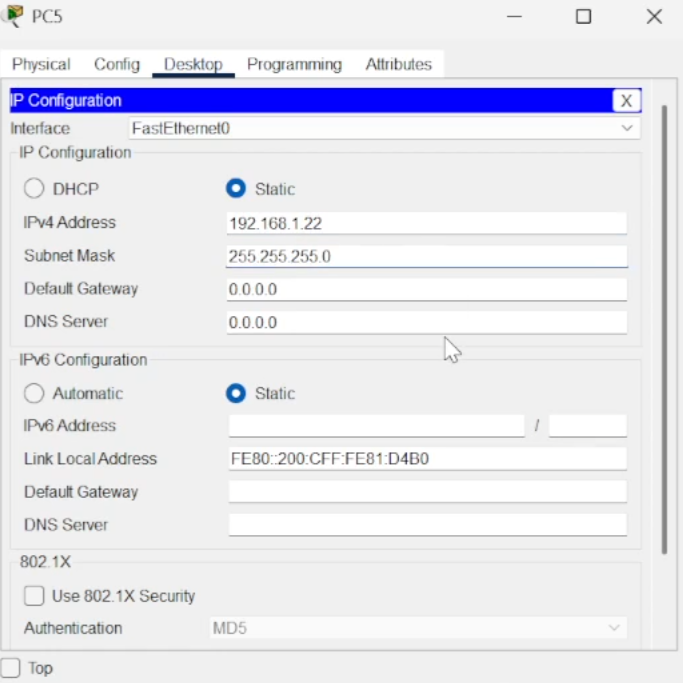
\includegraphics[width=\textwidth]{../images/17.png}
    \captionof{figure}{Статический IP-адрес для PC-PT PC5.}
    \label{17}
\end{center}
\begin{center}
    \centering
    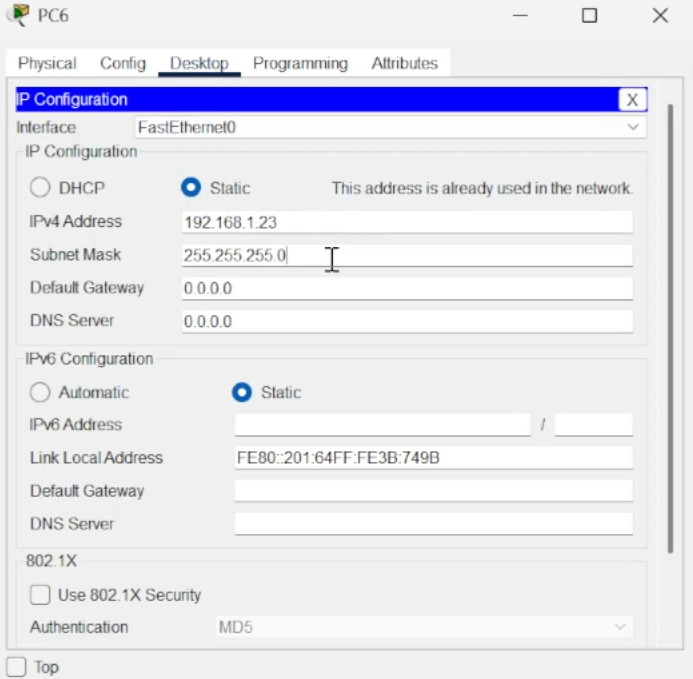
\includegraphics[width=\textwidth]{../images/18.png}
    \captionof{figure}{Статический IP-адрес для PC-PT PC6.}
    \label{18}
\end{center}
\begin{center}
    \centering
    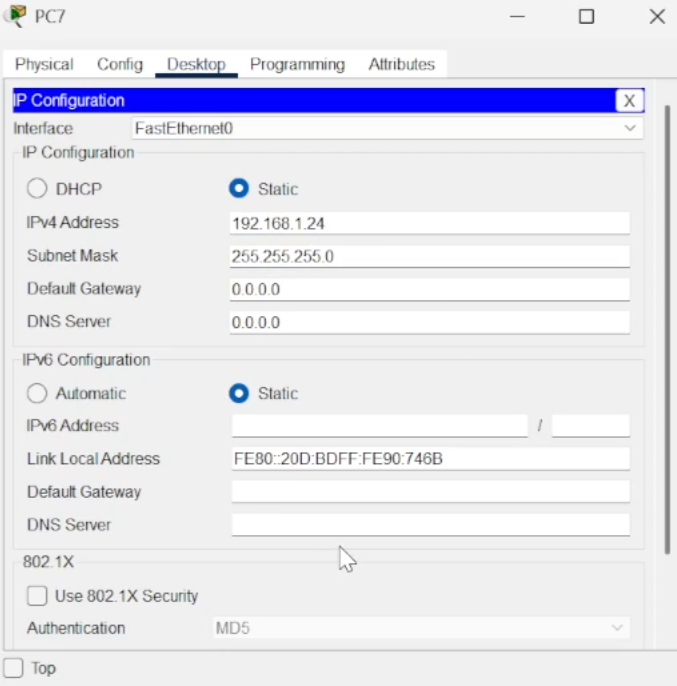
\includegraphics[width=\textwidth]{../images/19.png}
    \captionof{figure}{Статический IP-адрес для PC-PT PC7.}
    \label{19}
\end{center}

\item Переключимся из режима реального времени (Realtime) в режим моделирования (Simulation).

\item На панели инструментов выберем \textbf{«Add Simple PDU (P)»} и щёлкнем сначала на \textbf{PC4}, затем на \textbf{PC6}.

\item В рабочей области появятся два конверта (пакеты), в списке событий на панели моделирования отобразятся два события:
\begin{itemize}
    \item \textbf{ARP} — запрос MAC-адреса узла назначения;
    \item \textbf{ICMP} — Echo Request (ping).
\end{itemize}

\item На панели моделирования нажмём кнопку \textbf{«Play»} и проследим за движением пакетов ARP и ICMP от PC4 до PC6 и обратно (Рис. \ref{20}):

\begin{center}
    \centering
    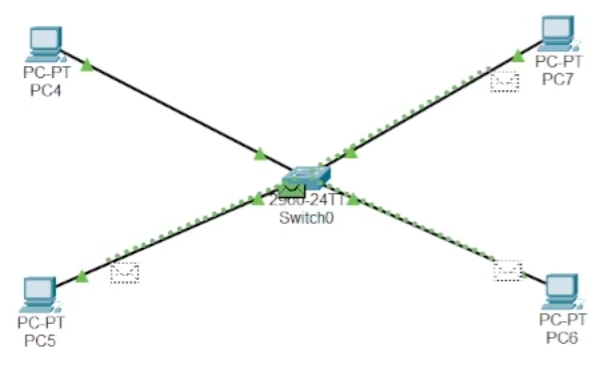
\includegraphics[width=0.8\textwidth]{../images/20.png}
    \captionof{figure}{Движение пакетов ARP и ICMP в сети с коммутатором.}
    \label{20}
\end{center}

\subsubsection*{Сравнительный анализ работы ARP: концентратора и коммутатора}
\begin{center}
\begin{tabular}{|p{4cm}|p{5cm}|p{5cm}|}
\hline
\textbf{Критерий} & \textbf{Концентратор (Hub-PT)} & \textbf{Коммутатор (Switch 2960)} \\
\hline
\textbf{Распространение ARP-запроса} & Широковещательный запрос передаётся на \textbf{все порты}, кроме входящего. & Широковещательный запрос передаётся на \textbf{все порты}, кроме входящего (флуд). \\
\hline
\textbf{Реакция на ARP-ответ} & Концентратор не изучает MAC-адреса. ARP-ответ передаётся на \textbf{все порты}, кроме входящего. & Коммутатор изучает Source MAC и добавляет запись в \textbf{CAM-таблицу}. ARP-ответ передаётся \textbf{только на порт отправителя}. \\
\hline
\textbf{Повторный ARP-запрос} & Снова широковещательная передача на все порты. & Если MAC-адрес уже есть в CAM-таблице, коммутатор передаёт кадр \textbf{только на целевой порт} (без флуда). \\
\hline
\textbf{Загрузка сети} & \textbf{Высокая} — все устройства в домене коллизий получают все кадры. & \textbf{Низкая} — кадры передаются только адресату (после изучения MAC). \\
\hline
\textbf{Домен коллизий} & \textbf{Один общий} домен коллизий. & \textbf{Отдельный} домен коллизий на каждый порт. \\
\hline
\textbf{Домен широковещания} & Один домен широковещания. & Один домен широковещания (без VLAN). \\
\hline
\end{tabular}
\end{center}

\subsubsection*{Структура кадра Ethernet для ICMP}
\textbf{Тип кадра:} \textbf{Ethernet II} (определяется по полю EtherType = 0x0800).

\begin{center}
\begin{tabular}{|l|l|c|}
\hline
\textbf{Поле} & \textbf{Значение} & \textbf{Длина} \\
\hline
Destination MAC & MAC-адрес получателя & 6 байт \\
Source MAC & MAC-адрес отправителя & 6 байт \\
EtherType & 0x0800 (IPv4) & 2 байта \\
Data & IP-пакет (ICMP внутри) & переменная \\
FCS & Контрольная сумма & 4 байта \\
\hline
\end{tabular}
\end{center}

\subsubsection*{Структура пакета ICMP (Echo Request / Echo Reply)}
\begin{center}
\begin{tabular}{|l|l|c|}
\hline
\textbf{Поле} & \textbf{Значение} & \textbf{Длина} \\
\hline
Type & 8 (Request) / 0 (Reply) & 1 байт \\
Code & 0 & 1 байт \\
Checksum & Контрольная сумма & 2 байта \\
Identifier & Идентификатор процесса & 2 байта \\
Sequence Number & Номер последовательности & 2 байта \\
Data & Произвольные данные (payload) & переменная \\
\hline
\end{tabular}
\end{center}

\subsubsection*{Структура MAC-адресов}
\begin{center}
\begin{tabular}{|l|l|l|}
\hline
\textbf{Тип MAC} & \textbf{Пример} & \textbf{Описание} \\
\hline
Destination MAC & 00:0C:29:AB:CD:EF & Адрес получателя (меняется при маршрутизации) \\
Source MAC & 00:60:5C:AD:5C:3B & Адрес отправителя (меняется при маршрутизации) \\
Broadcast MAC & FF:FF:FF:FF:FF:FF & Широковещательный (ARP-запрос) \\
Multicast MAC & 01:00:0C:CC:CC:CC & CDP (Cisco) \\
Multicast MAC & 01:80:C2:00:00:00 & STP BPDU \\
\hline
\end{tabular}
\end{center}

\subsubsection*{Изменения в кадре Ethernet при передвижении пакета}
\begin{itemize}
    \item \textbf{Внутри одной сети (L2-сегмент):} \\
    Destination MAC и Source MAC \textbf{не изменяются}. Коммутатор только пересылает кадр на целевой порт.
    \item \textbf{При прохождении через маршрутизатор (L3):} \\
    Destination MAC $\rightarrow$ меняется на MAC следующего hop'а. \\
    Source MAC $\rightarrow$ меняется на MAC исходящего интерфейса маршрутизатора. \\
    IP-адреса источника и назначения \textbf{не изменяются}, TTL уменьшается на 1.
\end{itemize}

\item Очистим список событий, удалив сценарий моделирования (Reset Simulation).

\item На панели инструментов выберем \textbf{«Add Simple PDU (P)»} и выполним:
\begin{itemize}
    \item Щёлкнем сначала на \textbf{PC4}, затем на \textbf{PC6}.
    \item Щёлкнем сначала на \textbf{PC6}, затем на \textbf{PC4}.
\end{itemize}

\item На панели моделирования нажмём кнопку \textbf{«Play»} и проследим за движением пакетов (Рис. \ref{21}):

\begin{center}
    \centering
    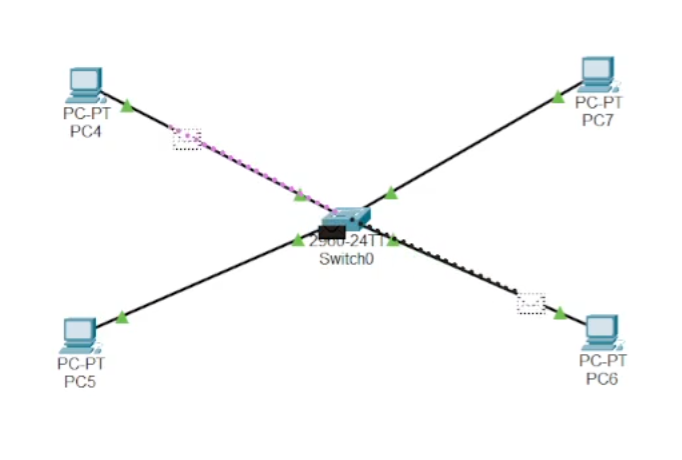
\includegraphics[width=0.8\textwidth]{../images/21.png}
    \captionof{figure}{Отсутствие коллизии.}
    \label{21}
\end{center}

\subsubsection*{Анализ отсутствия коллизии}
\textbf{Почему в данной схеме коллизия не возникает?}

В отличие от концентратора (Hub), коммутатор (Switch 2960) является устройством \textbf{канального уровня (L2)} с буферизацией кадров и технологией \textbf{store-and-forward}.

\subsubsection*{Причины отсутствия коллизии:}
\begin{enumerate}
    \item \textbf{Раздельные домены коллизий:}
    \begin{itemize}
        \item Каждый порт коммутатора — это \textbf{отдельный домен коллизий}.
        \item Пакеты от PC4 к PC6 и от PC6 к PC4 передаются \textbf{по разным физическим каналам}.
        \item Сигналы не накладываются друг на друга, так как среда передачи на каждом порту независима.
    \end{itemize}
    \item \textbf{Полнодуплексный режим:}
    \begin{itemize}
        \item Коммутатор и PC работают в \textbf{full-duplex} (одновременная передача и приём на одном порту).
        \item В полнодуплексном режиме \textbf{коллизии отсутствуют} по определению.
        \item Отключён механизм CSMA/CD.
    \end{itemize}
    \item \textbf{Буферизация кадров:}
    \begin{itemize}
        \item Коммутатор полностью принимает кадр в буфер, проверяет FCS, затем передаёт на целевой порт.
        \item Даже если два кадра приходят на разные порты одновременно, они оба буферизируются и передаются последовательно.
    \end{itemize}
    \item \textbf{Коммутация адресная:}
    \begin{itemize}
        \item После изучения MAC-адресов коммутатор отправляет кадры \textbf{только на целевой порт}, а не на все.
        \item Кадр от PC4 к PC6 идёт только на порт PC6, кадр от PC6 к PC4 — только на порт PC4.
        \item Эти потоки не пересекаются физически.
    \end{itemize}
\end{enumerate}

\subsubsection*{Сравнение с концентратором:}
\begin{center}
\begin{tabular}{|p{4cm}|p{5cm}|p{5cm}|}
\hline
\textbf{Параметр} & \textbf{Концентратор (Hub)} & \textbf{Коммутатор (Switch)} \\
\hline
Домен коллизий & Один общий & На каждый порт отдельный \\
Режим передачи & Полудуплекс (half-duplex) & Полный дуплекс (full-duplex) \\
Обработка кадров & Регенерация сигнала & Буферизация + коммутация \\
Коллизия при одновременной передаче & \textbf{Возникает} & \textbf{Не возникает} \\
\hline
\end{tabular}
\end{center}

\item Переключимся в режим реального времени (Realtime).

\item В рабочем пространстве соединим \textbf{кроссовым кабелем} (Copper Cross-Over) \textbf{концентратор (Hub-PT)} и \textbf{коммутатор (Switch 2960)} (Рис. \ref{22}):

\begin{center}
    \centering
    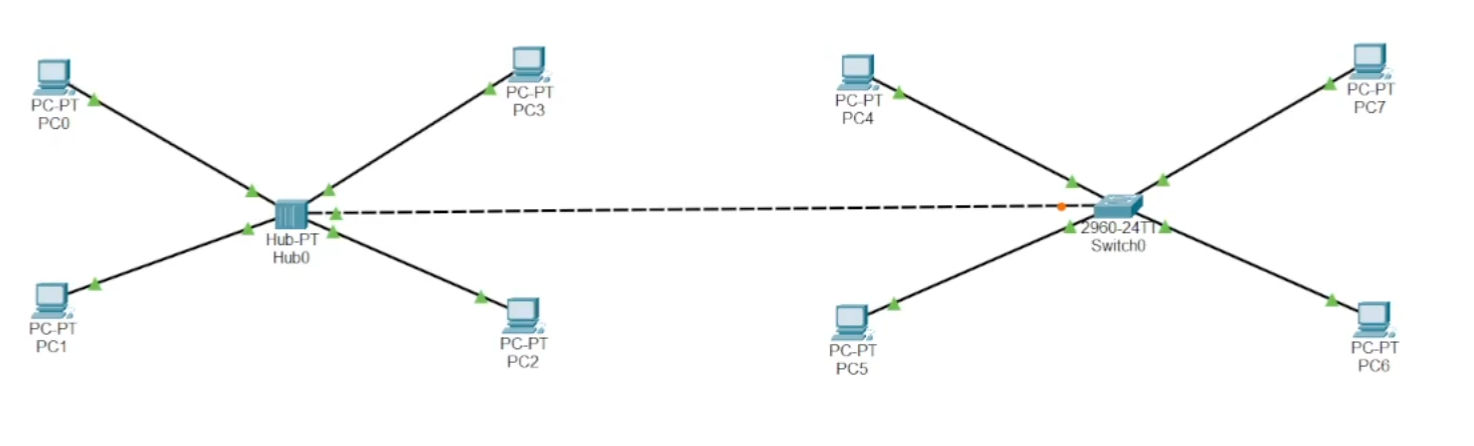
\includegraphics[width=0.8\textwidth]{../images/22.png}
    \captionof{figure}{Соединение двух схем.}
    \label{22}
\end{center}

\item Переключимся в режим моделирования (Simulation).

\item Очистим список событий (Reset Simulation).

\item На панели инструментов выберем \textbf{«Add Simple PDU (P)»} и выполним:
\begin{itemize}
    \item Щёлкнем сначала на \textbf{PC0}, затем на \textbf{PC4}.
    \item Щёлкнем сначала на \textbf{PC4}, затем на \textbf{PC0}.
\end{itemize}

\item На панели моделирования нажмём кнопку \textbf{«Play»} и проследим за движением пакетов (Рис. \ref{23}):

\begin{center}
    \centering
    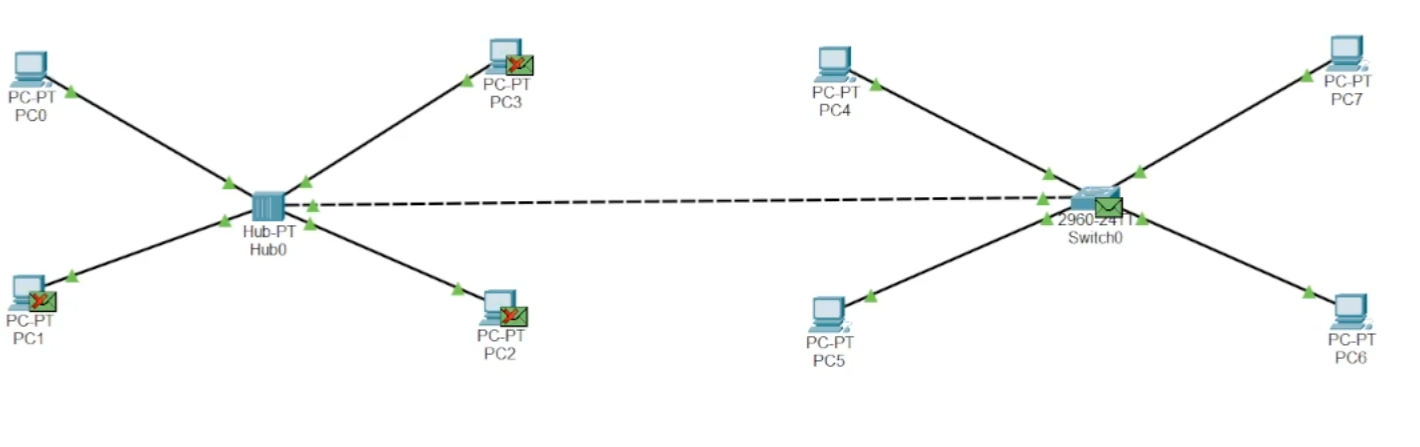
\includegraphics[width=0.8\textwidth]{../images/23.png}
    \captionof{figure}{Возникновение коллизии при передаче через концентратор и коммутатор.}
    \label{23}
\end{center}

\subsubsection*{Почему возникает коллизия?}
\textbf{Причина:} несимметричность сети и общий домен коллизий со стороны концентратора.

\begin{itemize}
    \item \textbf{PC0} и \textbf{PC1} находятся в сети концентратора (\textit{общий домен коллизий}).
    \item \textbf{PC4} и \textbf{PC6} находятся в сети коммутатора (\textit{раздельные домены коллизий}).
    \item Концентратор и коммутатор соединены кроссовым кабелем.
\end{itemize}

\textbf{Механизм возникновения коллизии:}
\begin{enumerate}
    \item \textbf{PC0} отправляет кадр в сторону \textbf{PC4}.
    \item \textbf{PC4} одновременно отправляет кадр в сторону \textbf{PC0}.
    \item Кадр от PC4 проходит через коммутатор (буферизация, полный дуплекс) и направляется в сторону концентратора.
    \item Кадр от PC0 проходит через концентратор и ретранслируется на \textbf{все порты}, включая порт, ведущий к коммутатору.
    \item На \textbf{сегменте между концентратором и коммутатором} происходит \textbf{наложение сигналов} (кадр от PC0 и кадр от PC4 встречаются).
    \item Возникает \textbf{коллизия}, кадры повреждаются.
\end{enumerate}

\subsubsection*{Почему затем пакеты успешно достигают цели?}
\textbf{Причина:} повторная передача после коллизии и изучение MAC-адресов коммутатором.

\begin{enumerate}
    \item После обнаружения коллизии оба устройства (\textbf{PC0} и \textbf{PC4}) ждут случайное время (\textbf{backoff} по алгоритму CSMA/CD).
    \item \textbf{PC0} повторяет отправку ARP-запроса.
    \item \textbf{Концентратор} ретранслирует ARP-запрос на все порты, включая порт к коммутатору.
    \item \textbf{Коммутатор} получает ARP-запрос, флудит его на все порты (кроме входящего).
    \item \textbf{PC4} отвечает ARP-ответом.
    \item \textbf{Коммутатор} изучает MAC-адрес PC4 и отправляет ARP-ответ \textbf{только на порт, ведущий к концентратору} (так как MAC-адрес PC0 уже изучен из ARP-запроса).
    \item ARP-ответ проходит через концентратор к PC0 без коллизии, так как PC4 в этот момент не передаёт.
    \item Далее ICMP-пакеты передаются уже по известным MAC-адресам.
\end{enumerate}

\subsection*{Исследование STP (Spanning Tree Protocol)}
\item Очистим список событий, удалив сценарий моделирования (Reset Simulation).

\item На панели моделирования нажмём кнопку \textbf{«Play»}. В списке событий получим пакеты \textbf{STP} (Рис. \ref{24}).

\begin{center}
    \centering
    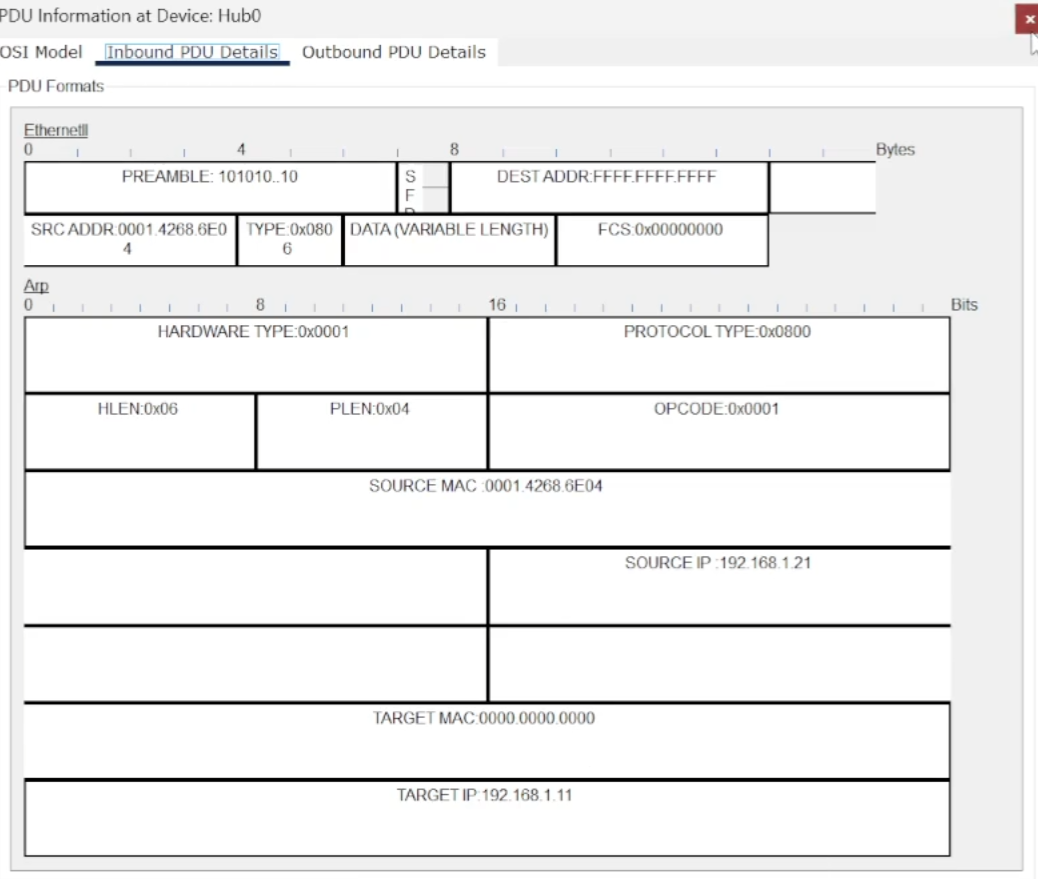
\includegraphics[width=0.8\textwidth]{../images/24.png}
    \captionof{figure}{Пакеты STP (BPDU) в списке событий.}
    \label{24}
\end{center}

\subsubsection*{Структура кадра Ethernet для STP BPDU}
\textbf{Тип кадра:} \textbf{IEEE 802.3 + LLC} (не Ethernet II!).

\begin{center}
\begin{tabular}{|l|l|c|}
\hline
\textbf{Поле} & \textbf{Значение} & \textbf{Длина} \\
\hline
PREAMBLE & 101010…10 & 7 байт \\
SFD & 10101011 & 1 байт \\
Destination MAC & 01:80:C2:00:00:00 & 6 байт \\
Source MAC & MAC-адрес порта коммутатора & 6 байт \\
Length & 38–1500 (обычно 38+) & 2 байта \\
LLC Header & DSAP=0x42, SSAP=0x42, Ctrl=0x03 & 3 байта \\
BPDU Data & STP Configuration / TCN BPDU & переменная \\
FCS & Контрольная сумма & 4 байта \\
\hline
\end{tabular}
\end{center}

\subsubsection*{Структура MAC-адресов STP}
\begin{center}
\begin{tabular}{|l|l|l|}
\hline
\textbf{Адрес} & \textbf{Значение} & \textbf{Описание} \\
\hline
Destination MAC & \texttt{01:80:C2:00:00:00} & Групповой адрес мостов (Bridge Group Address) \\
Source MAC & \texttt{00:0D:BD:F2:1A:40} & MAC-адрес порта коммутатора \\
\hline
\end{tabular}
\end{center}

\textbf{Важно:}
\begin{itemize}
    \item Адрес \texttt{01:80:C2:00:00:00} не пересылается другими мостами/коммутаторами (зарезервирован для протоколов L2).
    \item Кадр имеет поле \textbf{Length}, а не EtherType → это \textbf{802.3}.
    \item LLC указывает на протокол STP (0x42).
\end{itemize}

\subsection*{Добавление маршрутизатора}
\item Перейдём в режим реального времени (Realtime).

\item В рабочем пространстве добавим маршрутизатор \textbf{Cisco 2811} (категория Routers).

\item Соединим \textbf{прямым кабелем} (Copper Straight-Through) коммутатор и маршрутизатор.

\item Настроим маршрутизатор:
\begin{enumerate}
    \item Щёлкнем на \textbf{Router0} → вкладка \textbf{Config}.
    \item Выберем \textbf{INTERFACE} → \textbf{FastEthernet0/0}.
    \item \textbf{IP Address:} \texttt{192.168.1.254}
    \item \textbf{Subnet Mask:} \texttt{255.255.255.0}
    \item \textbf{Port Status:} \textbf{On}.
\end{enumerate}

\begin{center}
    \centering
    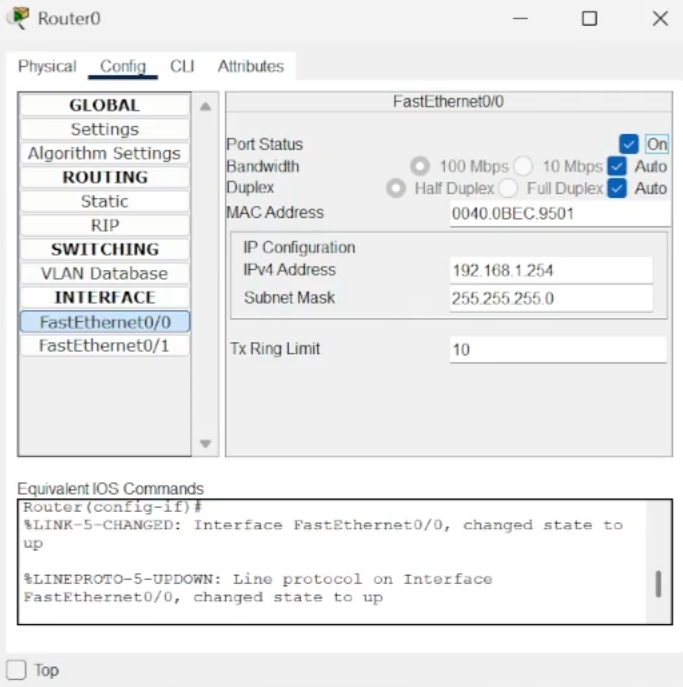
\includegraphics[width=0.8\textwidth]{../images/25.png}
    \captionof{figure}{Настройка IP-адреса на маршрутизаторе.}
    \label{25}
\end{center}

\subsection*{Моделирование и исследование CDP}
\item Переключимся в режим моделирования (Simulation).

\item Очистим список событий (Reset Simulation).

\item На панели инструментов выберем \textbf{«Add Simple PDU (P)»} и щёлкнем сначала на \textbf{PC3}, затем на \textbf{Router0}.

\item На панели моделирования нажмём \textbf{«Play»} и проследим за движением пакетов: \textbf{ARP, ICMP, STP, CDP}.

\subsubsection*{Структура кадра Ethernet для CDP}
\textbf{Тип кадра:} \textbf{Ethernet II} (определяется по полю EtherType).

\begin{center}
\begin{tabular}{|l|l|c|}
\hline
\textbf{Поле} & \textbf{Значение} & \textbf{Длина} \\
\hline
PREAMBLE & 101010…10 & 7 байт \\
SFD & 10101011 & 1 байт \\
Destination MAC & 01:00:0C:CC:CC:CC & 6 байт \\
Source MAC & MAC-адрес порта маршрутизатора & 6 байт \\
EtherType & 0x2000 (CDP) & 2 байта \\
Data (CDP payload) & TLVs: Device ID, Address, Port ID, Platform, Capabilities & переменная \\
FCS & Контрольная сумма & 4 байта \\
\hline
\end{tabular}
\end{center}

\subsubsection*{Структура MAC-адресов CDP}
\begin{center}
\begin{tabular}{|l|l|l|}
\hline
\textbf{Адрес} & \textbf{Значение} & \textbf{Описание} \\
\hline
Destination MAC & \texttt{01:00:0C:CC:CC:CC} & Мультикаст Cisco (CDP, VTP, DTP) \\
Source MAC & \texttt{00:14:69:5A:BC:12} & MAC-адрес интерфейса маршрутизатора \\
\hline
\end{tabular}
\end{center}

\subsubsection*{Структура CDP-пакета (TLV — Type/Length/Value)}
\begin{center}
\begin{tabular}{|l|l|c|}
\hline
\textbf{Поле} & \textbf{Значение} & \textbf{Длина} \\
\hline
Version & 1 или 2 & 1 байт \\
TTL & 180 секунд & 1 байт \\
Checksum & Контрольная сумма & 2 байта \\
\hline
\multicolumn{3}{|c|}{TLV (переменное число)} \\
\hline
Device ID TLV & Имя устройства (Router0) & переменная \\
Address TLV & IP-адрес (192.168.1.254) & переменная \\
Port ID TLV & FastEthernet0/0 & переменная \\
Capabilities TLV & Router & 4 байта \\
Platform TLV & Cisco 2811 & переменная \\
\hline
\end{tabular}
\end{center}

\subsection*{Сравнение типов кадров Ethernet}
\begin{center}
\begin{tabular}{|l|l|l|l|}
\hline
\textbf{Протокол} & \textbf{Тип кадра} & \textbf{Признак} & \textbf{Destination MAC} \\
\hline
STP (BPDU) & 802.3 + LLC & Length & 01:80:C2:00:00:00 \\
CDP & Ethernet II & EtherType = 0x2000 & 01:00:0C:CC:CC:CC \\
ARP & Ethernet II & EtherType = 0x0806 & FF:FF:FF:FF:FF:FF \\
ICMP (IPv4) & Ethernet II & EtherType = 0x0800 & MAC получателя \\
\hline
\end{tabular}
\end{center}

\end{enumerate}

\newpage
\section*{Общий вывод по лабораторной работе}

В ходе выполнения лабораторной работы были изучены принципы функционирования основных сетевых устройств — \textbf{концентратора (Hub)}, \textbf{коммутатора (Switch)} и \textbf{маршрутизатора (Router)} — а также протоколы \textbf{ARP}, \textbf{ICMP}, \textbf{STP} и \textbf{CDP} с использованием симулятора Cisco Packet Tracer.

\subsection*{1. Сравнительный анализ устройств}
\begin{itemize}
    \item \textbf{Концентратор (Hub)} — устройство физического уровня. Он не анализирует трафик, не буферизирует кадры и ретранслирует сигналы на все порты, кроме входящего. Это приводит к:
    \begin{itemize}
        \item единому домену коллизий;
        \item высокому уровню коллизий при одновременной передаче;
        \item неэффективному использованию пропускной способности;
        \item отсутствию механизмов изучения MAC-адресов.
    \end{itemize}
    
    \item \textbf{Коммутатор (Switch)} — устройство канального уровня. Он анализирует MAC-адреса, строит CAM-таблицу и передаёт кадры адресно. Это обеспечивает:
    \begin{itemize}
        \item раздельные домены коллизий на каждом порту;
        \item полнодуплексный режим передачи;
        \item отсутствие коллизий;
        \item эффективное использование полосы пропускания.
    \end{itemize}
    
    \item \textbf{Маршрутизатор (Router)} — устройство сетевого уровня. Он обеспечивает связь между различными IP-подсетями, изменяет MAC-адреса при передаче кадров и выполняет маршрутизацию на основе IP-адресов.
\end{itemize}

\subsection*{2. Протоколы и их особенности}
\begin{itemize}
    \item \textbf{ARP} — используется для разрешения IP-адресов в MAC-адреса. Широковещательный запрос, индивидуальный ответ. В сети с концентратором ARP-ответ видят все устройства, с коммутатором — только целевое.
    \item \textbf{ICMP} — протокол диагностики и сообщения об ошибках. Инкапсулируется в IP-пакет, затем в Ethernet-кадр типа Ethernet II (EtherType = 0x0800).
    \item \textbf{STP} — протокол предотвращения петель в сети с избыточными связями. Использует BPDU-кадры с мультикастовым MAC-адресом \texttt{01:80:C2:00:00:00} и типом кадра 802.3 + LLC.
    \item \textbf{CDP} — проприетарный протокол Cisco для обнаружения соседних устройств. Передаётся в кадрах Ethernet II с мультикастовым адресом \texttt{01:00:0C:CC:CC:CC} и EtherType = 0x2000.
\end{itemize}

\subsection*{3. Изменение MAC-адресов при передаче}
\begin{itemize}
    \item \textbf{Внутри одного L2-сегмента} (коммутатор, концентратор): MAC-адреса источника и назначения \textbf{не изменяются}.
    \item \textbf{При прохождении через маршрутизатор}:
    \begin{itemize}
        \item Source MAC заменяется на MAC исходящего интерфейса маршрутизатора;
        \item Destination MAC заменяется на MAC следующего hop'а;
        \item IP-адреса источника и назначения остаются неизменными;
        \item TTL уменьшается на 1.
    \end{itemize}
\end{itemize}

\subsection*{4. Коллизии и их предотвращение}
\begin{itemize}
    \item В сети с \textbf{концентратором} коллизии неизбежны при одновременной передаче нескольких устройств (единый домен коллизий, полудуплексный режим).
    \item В сети с \textbf{коммутатором} коллизии отсутствуют (раздельные домены коллизий, полнодуплексный режим, буферизация).
    \item В \textbf{гибридной сети} (Hub + Switch) коллизии возникают на сегменте между устройствами, так как порт коммутатора переключается в полудуплексный режим при подключении к концентратору. Повторная передача после коллизии обеспечивается алгоритмом CSMA/CD.
\end{itemize}

\subsection*{5. Типы кадров Ethernet}
\begin{itemize}
    \item \textbf{Ethernet II} — используется протоколами IP (0x0800), ARP (0x0806), CDP (0x2000). Определяется по полю \textbf{EtherType}.
    \item \textbf{IEEE 802.3 + LLC} — используется протоколом STP. Определяется по полю \textbf{Length}.
\end{itemize}

\subsection*{Заключение}
В результате выполнения лабораторной работы были получены практические навыки:
\begin{itemize}
    \item Построения сетевых топологий различной сложности;
    \item Настройки IP-адресации на оконечных устройствах и маршрутизаторах;
    \item Использования режимов Realtime и Simulation для анализа трафика;
    \item Исследования структуры кадров Ethernet и пакетов протоколов ARP, ICMP, STP, CDP;
\end{itemize}

\end{document}
